\def\SigleNumero{STT-2902}
\def\NomCours{Modélisation statistique}
\def\DateEvaluation{10 décembre 2025}
\def\HeureEvaluation{8 h 30 à 10 h 20}
\def\Session{}
\def\NomEvaluation{Examen 3}
\def\Ponderation{}
% Ne rien mettre entre les accolades si l'enseignant (ou l'enseignante) est aussi le coordonnateur (ou la coordonnatrice)
\def\Coordonnatrice{}
\def\Coordonnateur{}

% Ne rien mettre entre les accolades s'il y a plus d'une section
\def\Enseignant{Julien Miron}
\def\Enseignante{}

% Ne rien mettre entre les accolades s'il s'agit d'un cours à section unique
% Mettre le nom de chacun des enseignants et enseignantes entre les accolades
% Une case à cocher sera générée pour chacune des sections
\def\SectionA{}
\def\SectionB{}
\def\SectionC{}
\def\SectionD{}


\def\Directives{
\begin{enumerate}
\item Matériel autorisé:
\begin{itemize}
    \item Calculatrice scientifique {\bf autorisée par la faculté des sciences et de génie};
    \item Votre cahier de notes de cours;
    \end{itemize}
\item Assurez-vous que cette évaluation comporte \numquestions ~questions réparties sur \numpages{}~pages, pour un total de \numpoints{}~points et \numbonuspoints{}~points bonus.\
\item \textbf{Veuillez ne pas dégrafer votre examen.}
\item Ajoutez vos initiales dans le bas de chaque page.
\item Vous devez\textbf{ justifier toutes vos réponses} par une démarche claire, sauf pour les questions à choix de réponse.\
\item Pour les questions à choix de réponse et les vrais ou faux, vous pouvez mettre un X, un crochet ($\checkmark$) ou remplir la case.\
\item Certains vrais ou faux demandent une justification. Aucun point ne sera donné sans justification, même si vous cochez la bonne réponse.
\item Pour les questions à choix de réponse, lorsqu'il est écrit «cochez tous les énoncés qui sont vrais/faux», il est possible qu'un seul énoncé soit vrai.
\item Le verso des feuilles peut être utilisé comme brouillon, \textbf{mais ne sera pas corrigé}. Attention à ne rien dégrafer.
\end{enumerate}
}



\documentclass{Examens/Evaluation}
\usepackage{multicol,graphicx}
\begin{document}

\pageblanche
\begin{questions} 

\question[3] Dans un modèle de régression linéaire simple pour lequel $\beta_0=0$, quel est l'interprétation du paramètre $\beta_1$ ?

\begin{checkboxes}
    \choice La valeur moyenne de Y quand X = 1
\choice La différence entre $y_i$ et $y_j$ quand $x_i$ et $x_j$ sont distants de 1 unité
\choice L’erreur aléatoire du modèle
\choice La valeur prédite de Y pour n’importe quel X
\end{checkboxes}

\vspace{0.5cm}
\question[3] Pour faire de l’inférence sur $\beta_1$ dans le cadre de la régression linéaire simple, on doit notamment supposer que :

\begin{checkboxes}
    \choice Les $Y_i$ sont des variables aléatoires normales indépendantes d'espérance nulle et de variance constante.
\choice Les $\epsilon_i$ sont des variables aléatoires normales indépendantes d'espérance nulle et de variance constante.
\choice X doit suivre une loi normale
\choice Toutes les valeurs de X doivent être distinctes
\end{checkboxes}

\vspace{0.5cm}

\question[3] La statistique du khi-carré pour tester l’indépendance compare :

\begin{checkboxes}
\choice Les lois marginales entre elles
\choice Les fréquences observées aux fréquences attendues
\choice Les moyennes conditionnelles
\choice La variance de Y pour chaque valeur de X
\end{checkboxes}

\vspace{0.5cm}
\question Soit l'intervalle de confiance de niveau $95\%$ pour $\beta_1$: $[2,5; 6,9]$.
\begin{parts}
\vspace{0.5cm}
    \part[1] Nous savons que $\widehat{\beta}_1=5,7$.
    
    \begin{oneparcheckboxes}
        \choice Vrai
        \choice Faux
    \end{oneparcheckboxes}

\vspace{0.5cm}
    \part[1] Nous rejetons $H_0:\beta_1=0$ au profit de $H_1:\beta_1\neq 0$ au seuil $5\%$.
        
    \begin{oneparcheckboxes}
        \choice Vrai
        \choice Faux
    \end{oneparcheckboxes}

\vspace{0.5cm}
\part[1] Nous rejetons $H_0:\beta_1=0$ au profit de $H_1:\beta_1\neq 0$ au seuil $10\%$.

        \begin{oneparcheckboxes}
        \choice Vrai
        \choice Faux
    \end{oneparcheckboxes}
    
\end{parts}

\vspace{0.5cm}

\question D'au moins combien de paires d'observations avons-nous besoin pour pouvoir utiliser chacune des méthodes suivantes?

\vspace{0.5cm}
\begin{parts}
    \part[1] Méthode de Mayer
    
    \begin{oneparcheckboxes}
        \choice 0
        \choice 1
        \choice 2
        \choice 3
        \choice 4+
    \end{oneparcheckboxes}

\vspace{0.5cm}

     \part[1] Méthode Med-Med
    
    \begin{oneparcheckboxes}
        \choice 0
        \choice 1
        \choice 2
        \choice 3
        \choice 4+
    \end{oneparcheckboxes}

\vspace{0.5cm}

     \part[1] Méthode des moindres carrés (estimation et inférence incluses)
    
    \begin{oneparcheckboxes}
        \choice 0
        \choice 1
        \choice 2
        \choice 3
        \choice 4+
    \end{oneparcheckboxes}
\end{parts}
\pageblanche
%%%%%%%%%%%%%%%% QUESTION %%%%%%%%%%%%%%%%

\question\label{rls} Soit le graphique suivant qui représente les observations $(x_1,y_1),\hdots,(x_9, y_9)$.

\begin{center}
    
% --- À mettre dans un document LaTeX avec \usepackage{tikz} ---
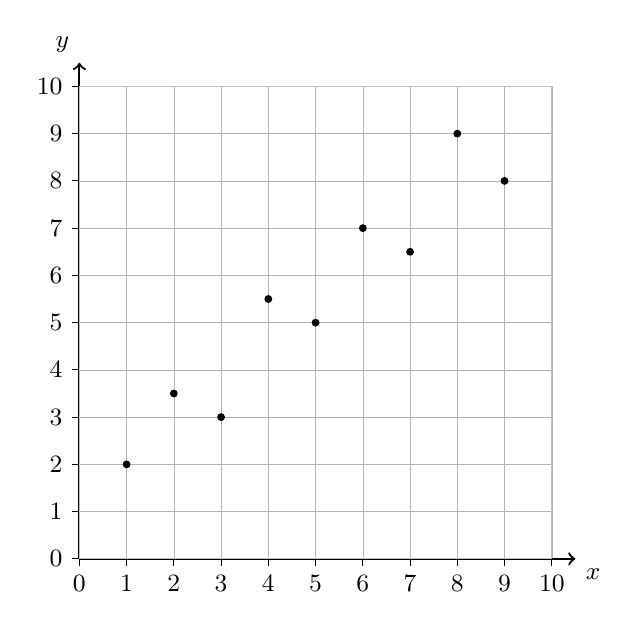
\begin{tikzpicture}[scale=0.6]
  % Styles
  \tikzset{
    pt/.style={fill=black, draw=black, circle, minimum size=4pt, inner sep=0pt},
    axe/.style={->, thick},
  }

  % Grille de fond
  \draw[very thin, color=gray!60, step=1] (0,0) grid (10,10);

  % Axes
  \draw[axe] (0,0) -- (10.5,0) node[below right]{\small $x$};
  \draw[axe] (0,0) -- (0,10.5) node[above left]{\small $y$};

  % Graduations
  \foreach \x in {0,...,10}
    \draw (\x,0) -- (\x,-0.15) node[below] {\small \x};
  \foreach \y in {0,...,10}
    \draw (0,\y) -- (-0.15,\y) node[left] {\small \y};

  % Cadre extérieur
  \draw[gray!50] (0,0) rectangle (10,10);

  % Points (à modifier si tu veux d'autres coordonnées)
  \foreach \x/\y in {
    1/2,
    2/3.5,
    3/3,
    4/5.5,
    5/5,
    6/7,
    7/6.5,
    8/9,
    9/8
  }{
    \filldraw[pt] (\x,\y) circle (2pt);
    % Si tu veux afficher les coordonnées :
    % \node[above left,font=\footnotesize] at (\x,\y) {(\x,\y)};
  }

\end{tikzpicture}
\end{center}

\begin{parts}
    \part[3] Estimez la droite de régression à l'aide de la méthode de Mayer.

    \vspace{8cm}

    \part[3] Estimez la droite de régression à l'aide de la méthode Médiane-Médiane.

\vfill
\pagesuivante{\ref{rls}}
    \pageblanche
\suite{\ref{rls}}
    \part[5]\label{estmc} En utilisant les mêmes données et les informations ci-dessous, donnez l'estimation de la droite de régression à l'aide de la méthodes des moindres carrés.

    \begin{align*}
        \sum_{i=1}^9x_i=36 &&\sum_{i=1}^9x_i^2=285 && \sum_{i=1}^9y_i=49,5 & & \sum_{i=1}^9x_iy_i=296,5 \\
    \end{align*}

\vfill
\pagesuivante{\ref{rls}}
    \pageblanche
\suite{\ref{rls}}

    \part[4] Complétez le tableau suivant à l'aide de la droite estimée en (\ref{estmc}). Si vous n'avez pas trouvé de valeurs en (\ref{estmc}), utilisez $\hat{\beta}_0=1$ et $\hat{\beta}_1=1$.

    \renewcommand{\arraystretch}{4} % augmente la hauteur et centre verticalement

\begin{table}[h]
    \centering
    \begin{tabular}{|>{\centering\arraybackslash}p{1.2cm}|
                    >{\centering\arraybackslash}p{1.2cm}|
                    >{\centering\arraybackslash}p{3cm}|
                    >{\centering\arraybackslash}p{3cm}|}
    \hline
    $x_i$ & $y_i$ & $\hat{y}_i$ & $\hat{\epsilon}_i$ \\
    \hline
    \hline
    1 & 2 & & \\ \hline
    2 & 3,5 & & \\ \hline
    3 & 3 & & \\ \hline
    4 & 5,5 & & \\ \hline
    5 & 5 & & \\ \hline
    6 & 7 & & \\ \hline
    7 & 6,5 & & \\ \hline
    8 & 9 & & \\ \hline
    9 & 8 & & \\ 
    \hline
    \end{tabular}
\end{table}



\part[4] Donnez la valeur de $MSE$.
\vfill
\pagesuivante{\ref{rls}}
\pageblanche
\suite{\ref{rls}}

\part[4] Donnez l'intervalle de confiance à $95\%$ pour $\beta_1$.

\vfill

\part[3] Donnez une interprétation de l'intervalle de confiance que vous venez de calculer.

\vspace{7cm}


\end{parts}

\pageblanche

\question\label{asso} Pour une étude de marché, on s'intéresse aux gens qui commandent les «Bénés du Tourne-Gaufre», la «Poutine Bon Matin» ou «L'Assiette Brunch» au restaurant \textit{Les Fraises du Tourne-Gaufre}.
Parmi ces gens, on veut savoir combien consomme de l'eau chaude avec du miel pour soulager la toux.
On obtient le tableau de fréquence suivant, où on utilise la lettre $X$ pour le choix de repas et la lettre $Y$ pour la consommation d'eau chaude avec du miel:

\renewcommand{\arraystretch}{2} % augmente la hauteur et centre verticalement

\begin{table}[h]
    \centering
    \begin{tabular}{|P{3cm}|P{2cm}|P{2cm}|}
    \hline
        \diagbox[innerwidth=3cm]{X}{Y} & Oui & Non \\
        \hline
         Bénés & 24 & 3\\
         \hline
         Poutine & 18 & 3\\
         \hline
         Assiette Brunch & 36 & 1\\
         \hline
    \end{tabular}

\end{table}

\begin{parts}
    \part[4] Remplissez le tableau suivant avec les valeurs \textit{attendues} si $X$ et $Y$ étaient indépendantes. Vous devez inclure sous le tableau la façon de calculer les valeurs en explicitant le calcul d'une des valeurs.

    \renewcommand{\arraystretch}{4} % augmente la hauteur et centre verticalement

\begin{table}[h]
    \centering
    \begin{tabular}{|P{3cm}|P{2cm}|P{2cm}|}
    \hline
        \diagbox[innerwidth=3cm]{X}{Y} & Oui & Non \\
        \hline
         Bénés &  & \\
         \hline
         Poutine &  & \\
         \hline
         Assiette Brunch &  & \\
         \hline
    \end{tabular}

\end{table}


\vfill
\pagesuivante{\ref{asso}}
\pageblanche
\suite{\ref{asso}}

\part[5] Procédez au test d'indépendance pour les variables $X$ et $Y$, au seuil $5\%$.


\end{parts}
\pageblanche

\question Soit les variables aléatoires $X$ et $Y$.
Voici le tableau qui représente la fonction de probabilité conjointe de $(X, Y)$ où $a$ et $b$ sont des probabilités.

\begin{center}
\large{
\begin{tabular}{cc|cccc}
$p(x,y)$ & & & $y$& &\\
 & & 0 & 1 & 2 &3 \\ 
 \hline
 & -1 & $a$ & $\sfrac{10}{110}$  & $\sfrac{14}{110}$ & $b$\\
$x$ & 2 & $\sfrac{23}{110}$ & $\sfrac{9}{110}$ & $\sfrac{1}{110}$& $\sfrac{30}{110}$\\
& 4 & $\sfrac{3}{110}$ & $0$ & $\sfrac{3}{110}$& $\sfrac{9}{110}$\\
\end{tabular}
}
 \end{center}
\vspace{0.25cm}\vspace{0.25cm}
 On sait que $P(X=-1)=\displaystyle \frac{32}{110}$ et $P(Y=3)=\displaystyle \frac{42}{110}$.
\vspace{0.25cm}
 \begin{parts}
     \part[3] Que valent $a$ et $b$?

     \vspace{5cm}

     \part[4]  Est-ce que $X$ et $Y$ sont indépendantes? Justifier votre réponse.
     
     \begin{oneparcheckboxes}
         \choice Oui
         \choice Non
     \end{oneparcheckboxes}

\vspace{3cm}

\part[3] Calculez $P(Y=2|X=2)$.
\end{parts}

\pageblanche
\bonusquestion[2] Avec $n=30$, nous faisons un test au seuil $\alpha$ pour confronter $H_0:\beta_1=0$ et $H_1:\beta_1\neq0$, et nous obtenons la statistique $\kappa_{obs}$. Tracez un graphique qui représente la situation où nous rejetons $H_0$. Il s'agit ici de tracer (rapidement) la densité de $\kappa_{obs}$ - \textit{identifiez bien sa loi!} - ainsi que d'ajouter la statistique observée du test et la valeur critique (ou la zone de rejet).

\vspace{10cm}
\bonusquestion[2] Dessinez le Père Noël. Ou quelque chose d'autre de votre choix. 







\end{questions}

\end{document} 
